\documentclass{amsart}
\usepackage[foot]{amsaddr} % put addresses on first page

\usepackage{geometry}
\usepackage{booktabs}
\usepackage{graphicx,psfrag,epsf}
\usepackage{enumerate}
\usepackage{enumitem}
\usepackage{amsfonts}
\usepackage{mathtools}
\usepackage{amssymb}
\usepackage{amsmath}
\allowdisplaybreaks
\usepackage{longtable}
\usepackage{bigints}
\usepackage{siunitx}
\usepackage{amsthm}
\usepackage{soul}
\usepackage{color}

\usepackage{hyperref}
\usepackage[capitalise]{cleveref}
\newtheorem{theorem}{Theorem}[section]
\newtheorem{corollary}{Corollary}[theorem]
\newtheorem{lemma}[theorem]{Lemma}
%

\usepackage[numbers]{natbib}
\usepackage{url} % not crucial - just used below for the URL 
\usepackage{doi}

\title{Copula estimation using loss-based Bayesian Additive Regression Trees}
\author{**}
\date{\today}

\begin{document}

\maketitle

\section{Introduction}

\section{Model}

\subsection{Conditional copula}

Let $Y_1$ and $Y_2$ be two continuous random variables and $X$ be a continuous random variable 
that might affect the relationship between $Y_1$ and $Y_2$. 
Then according to Sklar’s theorem there exists a unique copula such that:
\begin{equation}
    H_{X}(y_1,y_2\mid x; \theta, \alpha_1, \alpha_2) = C\{F_{Y_1\mid X}(y_1\mid x;\alpha_1),F_{Y_2\mid X}(y_2\mid x; \alpha_2)\mid x;\theta\}; \quad \forall (y_1,y_2) \in \mathbb{R}^2.
\end{equation}
This gives us the following
\begin{equation}
    h_{X}(y_1,y_2\mid x; \theta, \alpha_1, \alpha_2) = f_{Y_1\mid X}(y_1\mid x;\alpha_1)f_{Y_2\mid X}(y_2\mid x; \alpha_2)c(u_1,u_2\mid x;\theta),
\end{equation}
where
\begin{equation}\label{eq:emp_dist:Y}
    u_k = F_{Y_k\mid X}(y_k\mid x; \alpha_k)
\end{equation}
and $c(u_1,u_2\mid x;\theta)$ is conditional copula density function.

\subsection{Loss-based BART}

Let $T$ denote a tree and $M$ denote the vector of terminal node values $M = \{\mu_1,\mu_2, \cdots, \mu_{n_L}\}$. Let $\theta_i$ denote the copula parameter conditional on $x_i$ such that:
\begin{equation}
	\theta_i = g(x_i, T, M).
\end{equation}
For, $T,M$ a loss-based prior is proposed by \citet{serafini2024lossbasedpriortreetopologies} in the following way:
\begin{align}
	T, M &\sim \pi(T)\pi(M\mid T)\\
	T &\propto \exp\left(\omega n_L(T)-\gamma\Delta(T)\right)\\
	\pi(M\mid T) & = \prod_{j=1}^{n_L}\pi(\mu_j\mid T)
\end{align}

For the choice of prior on $\mu_j\mid T$ a conjugate prior is suggested by \citet{chipman_BART,serafini2024lossbasedpriortreetopologies}. However, finding a conjugate prior for copula parameter may not be possible always. Instead, we use a flat-prior on the support of the copula parameter and use a Metropolis-Hastings algorithm for obtaining posterior estimates.


\iffalse

\subsubsection{Choice for $\mu_j$}
\begin{itemize}
    \item Jeffrey's prior \url{https://www2.stat.duke.edu/~berger/papers/bivariate.pdf}
    \item Simple uniform distribution in $(-1,1)$ 
    \item Transformed beta \url{https://academic.oup.com/jrsssa/article/145/2/237/7105492}
    \item Log-normal on $-\log(1-p^2)$
    \item Inverse-Gamma on $-\log(1-p^2)$
\end{itemize}
Note that for the first three choices, we only work with transformed beta distribution by 
selecting suitable hyper-parameters.

\subsection{Density of $\rho$}

Let $\kappa = -\log(1-p^2)$, then for $\rho \ge 0$
\begin{align}
	\rho & = \sqrt{1-\exp(-\kappa)}\coloneqq g(\kappa)
\end{align}

Now, let $0\le\kappa_1 < \kappa_2<\infty$, then

\begin{align}
	&g(\kappa_2) - g(\kappa_1)\\
	&=\sqrt{1-\exp(-\kappa_2)} - \sqrt{1-\exp(-\kappa_1)}\\
	&= \frac{(\sqrt{1-\exp(-\kappa_2)} - \sqrt{1-\exp(-\kappa_1)})(\sqrt{1-\exp(-\kappa_2)} + \sqrt{1-\exp(-\kappa_1)})}{(\sqrt{1-\exp(-\kappa_2)} + \sqrt{1-\exp(-\kappa_1)})}\\
	&= \frac{(1-\exp(-\kappa_2) - 1+\exp(-\kappa_1))}{(\sqrt{1-\exp(-\kappa_2)} + \sqrt{1-\exp(-\kappa_1)})}\\
	&= \frac{(\exp(-\kappa_1)-\exp(-\kappa_2))}{(\sqrt{1-\exp(-\kappa_2)} + \sqrt{1-\exp(-\kappa_1)})}\\
	&= \frac{(\exp(\kappa_2)-\exp(-\kappa_1))}
	{(\exp(\kappa_2)\exp(-\kappa_1))(\sqrt{1-\exp(-\kappa_2)} + \sqrt{1-\exp(-\kappa_1)})} >0.
\end{align}
Therefore it is monotone and increasing.

Now, for $\rho \ge 0$ the density is given by
\begin{align}
	f_{\rho}(\rho)&=f_{\kappa}(\kappa)\left|\frac{d \kappa}{d \rho}\right|\\
	&=f_{\kappa}\left(-\log(1-p^2)\right)\frac{2\rho}{1-\rho^2}
\end{align}
Therefore for log-normal distribution
\begin{equation}
	f_{\rho}(\rho)
	= \frac{1}{\sqrt{2\pi\sigma^2}(-\log(1-\rho^2))} 
	\exp\left(-\frac{(\log(-\log(1-\rho^2))-\mu)^2}{2\sigma^2}\right)
	\cdot \frac{2\rho}{1-\rho^2}
\end{equation}
Similarly, we can derive the expression $\rho<0$ using the relation
$\rho = -\sqrt{1-\exp(-\kappa)}$. This gives us the following
symmetric density function
\begin{equation}
	f_{\rho}(\rho)
	= \frac{\sqrt{2}|\rho|}{\sqrt{\pi}\sigma(1-\rho^2)(-\log(1-\rho^2))} 
	\exp\left(-\frac{(\log(-\log(1-\rho^2))-\mu)^2}{2\sigma^2}\right)
\end{equation}

\paragraph{Continuity at 0} To show the continuity of the density function at 0 we first need to show that the limit $f_{\rho}(0)$
exists.

Since,

\begin{align}
	\lim_{\rho\to 0}f_{\rho}(\rho)
	&= \lim_{\rho\to 0}\left[\frac{\sqrt{2}|\rho|}{\sqrt{\pi}\sigma(1-\rho^2)(-\log(1-\rho^2))} 
	\exp\left(-\frac{(\log(-\log(1-\rho^2))-\mu)^2}{2\sigma^2}\right)\right]\\
	&= \frac{\sqrt{2}}{\sqrt{\pi}\sigma}\lim_{\rho\to 0}\left[\frac{|\rho|}{(1-\rho^2)} \right]
	\lim_{\rho\to 0}\left[\frac{1}{(-\log(1-\rho^2))} 
	\exp\left(-\frac{(\log(-\log(1-\rho^2))-\mu)^2}{2\sigma^2}\right)\right]
\end{align}
The limit $\lim_{\rho\to 0}\left[\frac{|\rho|}{(1-\rho^2)} \right]$ exists and equal to zero. For the remaining part we use change of variables.

\begin{align}
	&\lim_{\rho\to 0}\left[\frac{1}{(-\log(1-\rho^2))} 
	\exp\left(-\frac{(\log(-\log(1-\rho^2))-\mu)^2}{2\sigma^2}\right)\right]\\
	& = \lim_{\kappa\to 0}\left[\frac{1}{\kappa} 
	\exp\left(-\frac{(\log(\kappa)-\mu)^2}{2\sigma^2}\right)\right]\\
	& = \lim_{\eta\to -\infty}\left[\frac{1}{\exp(\eta)} 
	\exp\left(-\frac{(\eta-\mu)^2}{2\sigma^2}\right)\right]\\
	& = \lim_{\eta\to -\infty}\left[\frac{1}{\exp(\eta)} 
	\exp\left(-\frac{(\eta-\mu)^2}{2\sigma^2}\right)\right]\quad \text{TB: this holds for finite limits need to verify infinite}\\
	& = \lim_{\eta\to -\infty}\left[ 
	\exp\left(-\frac{(\eta-\mu)^2}{2\sigma^2}-\eta\right)\right] = 0
\end{align}
Since the density function is symmetric around 0, proceeding like before we can show that
\begin{equation}
	\lim_{\rho\to 0+}f_{\rho}(\rho) = \lim_{\rho\to 0-}f_{\rho}(\rho) = 0
\end{equation}

Now, for inverse-gamma distribution, the density of $\kappa$ is given by:
\begin{equation}
	f_{\kappa}(\kappa)= \frac{b^{a}}{\Gamma(a)}
	\kappa^{-a-1}\exp(-b/\kappa)
\end{equation}
Therefore, the density of $\rho$ is given by:
\begin{equation}
	f_{\rho}(\rho) = \frac{2b^{a}|\rho|}{\Gamma(a)(1-\rho^2)}
	(-\log(1-p^2))^{-a-1}\exp\left(-\frac{b}{-\log(1-p^2)}\right)
\end{equation}
Like before, we can show that the function is continuous at 0.

\begin{figure}[ht]
	\centering
	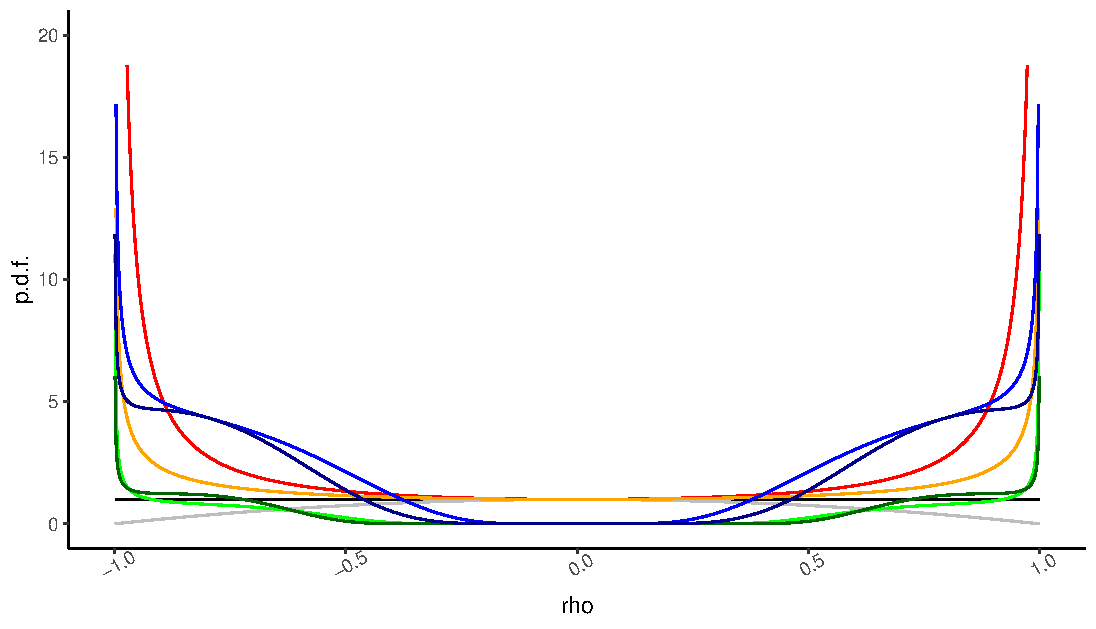
\includegraphics[width=0.85\linewidth]{prior_comparison.pdf}
	\caption{Different probability density functions for $\mu_j$ a)black for uniform distribution,
	b)grey for Beta(2,2),
	c)red for Jeffrey's prior,
	d)orange for Beta(0.5,0.5),
	e)green for inverse-gamma (1,1),
	f)dark green for inverse-gamma (2,2),
	g)blue for log-normal (0,1) and
	h)dark blue for log-normal (0, 0.8)}
	\label{fig:sim-prior}
\end{figure}
\fi

\section{Simulation Studies}

\subsection{Data generation}

To generate the true copula parameter, we first consider 4 different test cases to simulate Kendall's tau conditional on $x$. Such that
 
\begin{itemize}
    \item Case 1: True $\tau_x$ has a tree structure with respect to $x$.
    \item Case 2: True $\tau_x$ is monotone with respect to $x$ such that 
    \begin{equation}\label{eq:synth:tau_x:case2}
        \tau_x = 0.3 + 0.2 \sin(3x) + 0.3x^2.
    \end{equation}
    \item Case 3: True $\tau_x$ is convex with respect to $x$ such that 
    \begin{equation}\label{eq:synth:tau_x:case3}
        \tau_x = 0.5 + 0.3 \sin(3x).
    \end{equation}
    \item Case 4: True $\tau_x$ non-convex and non-monotone with respect to $x$ such that 
    \begin{equation}\label{eq:synth:tau_x:case4}
        \tau_x = 0.6 - 0.3 \sin(2x) + 0.2 \sin(4x) + 0.3 x^2.
    \end{equation}
\end{itemize}

Then using this value of conditional dependence, we can generate the copula parameters summarised in \cref{tab:cop:link}.

\begin{table}
    \centering
    \begin{tabular}{l|c|c}
    \toprule
        Family & Support & Relation with $\tau$ \\
         \midrule
        Gaussian & $\rho \in (-1,1)$ & $\sin(\tau\pi/2)$ \\
        Student-t & $\rho \in (-1,1)$ & $\sin(\tau\pi/2)$ \\
        Clayton & $\theta \in (0,\infty)$ & $2\tau/(1-\tau)$; $\tau>0$ \\
        Gumbel & $\theta\in [1,\infty)$ & $1/(1-\tau)$ \\
        \bottomrule
    \end{tabular}
    \caption{Copula family used for analysis, along with parameter support and relation with Kendall's $\tau$.}
    \label{tab:cop:link}
\end{table}

\subsection{Results}

\subsubsection{Gaussian Copula} For the Gaussian copula, the copula parameter $\rho$ lies within the open interval $(-1,1)$. So a natural choice for prior on $\mu_j$ is transformed beta as suggested by \citet{gokhale_prior_cor}. 

\begin{equation}
	\text{TBeta}(a, b) = \frac{1}{2^{a+b-1}\mathcal{B}(a,b)}(1+\rho)^{a-1}(1-\rho)^{b-1},
\end{equation}
for $a,b>0$ and $\mathcal{B}$ denotes beta function. Note that, for $a=b=0$, this leads to an improper prior. 

We present the summary of our analyses with Gaussian copula in \cref{tab:gauss:summary}. 

\begin{table}[ht]
	\centering
	\caption{Summary of analyses with Gaussian copula. The columns represents the specific case, the type of prior on $\mu_j\mid T$, the posterior expected number of terminal nodes, the posterior expected depth, the acceptance rate of MH algorithm, RMSE of estimated $\rho$ against true $\rho$, length of credible interval and coverage frequency within the credible interval. The posterior quantities are obtained by running 15000 samples in a single chain, after that we remove 5000 samples and then by thinned by 10.}
	\label{tab:gauss:summary}
	\scriptsize{
	\begin{tabular}{ll|cccccc}
		\toprule
		& Prior on $\mu_j$ & $\mathbb{E}(n_L\mid U,X)$ & $\mathbb{E}(D\mid U,X)$ & Acc. Rate & RMSE & CI length & CI coverage \\ 
		\midrule
		Case 1 & TBeta(0.5,0.5) & 4.538 & 2.403 & 0.2390 & 0.0096 & 0.1771 & 0.836 \\ 
		(Tree) & TBeta(0,0) & 4.862 & 2.607 & 0.2560 & 0.0089 & 0.1907 & 0.840 \\ 
		& TBeta(2,2) & 4.563 & 2.424 & 0.2420 & 0.0098 & 0.1948 & \textbf{0.908} \\ 
		& TBeta(1,1) & 4.608 & 2.484 & 0.2510 & 0.0092 & 0.1963 & 0.844 \\ 
		\midrule
		Case 2 & TBeta(0.5,0.5) & 3.176 & 1.814 & 0.2290 & 0.0021 & 0.1891 & 0.960 \\ 
		(\cref{eq:synth:tau_x:case2}) & TBeta(0,0) & 2.371 & 1.300 & 0.2130 & 0.0020 & 0.1592 & 0.968 \\ 
		& TBeta(2,2) & 2.522 & 1.390 & 0.2150 & 0.0020 & 0.1823 & \textbf{1.000} \\ 
		& TBeta(1,1) & 2.397 & 1.306 & 0.1900 & 0.0020 & 0.1625 & 0.930 \\ 
		\midrule
		Case 3 & TBeta(0.5,0.5) & 3.495 & 2.079 & 0.2410 & 0.0010 & 0.0743 & 0.760 \\ 
		(\cref{eq:synth:tau_x:case3}) & TBeta(0,0) & 3.863 & 2.165 & 0.2620 & 0.0009 & 0.0790 & \textbf{0.866} \\ 
		& TBeta(2,2) & 3.596 & 2.142 & 0.2460 & 0.0008 & 0.0808 & 0.790 \\ 
		& TBeta(1,1) & 5.374 & 2.966 & 0.3510 & 0.0009 & 0.0863 & 0.776 \\ 
		\midrule
		Case 4 & TBeta(0.5,0.5) & 2.558 & 1.402 & 0.2190 & 0.0005 & 0.1197 & \textbf{1.000} \\ 
		(\cref{eq:synth:tau_x:case4}) & TBeta(0,0) & 2.934 & 1.632 & 0.2520 & 0.0006 & 0.1227 & 0.972 \\ 
		& TBeta(2,2) & 2.398 & 1.308 & 0.2390 & 0.0005 & 0.1160 & 0.998 \\ 
		& TBeta(1,1) & 2.848 & 1.571 & 0.2120 & 0.0006 & 0.1296 & \textbf{1.000} \\ 
		\end{tabular}}
\end{table}


\paragraph{Trace-plots}

\begin{figure}
	\centering
	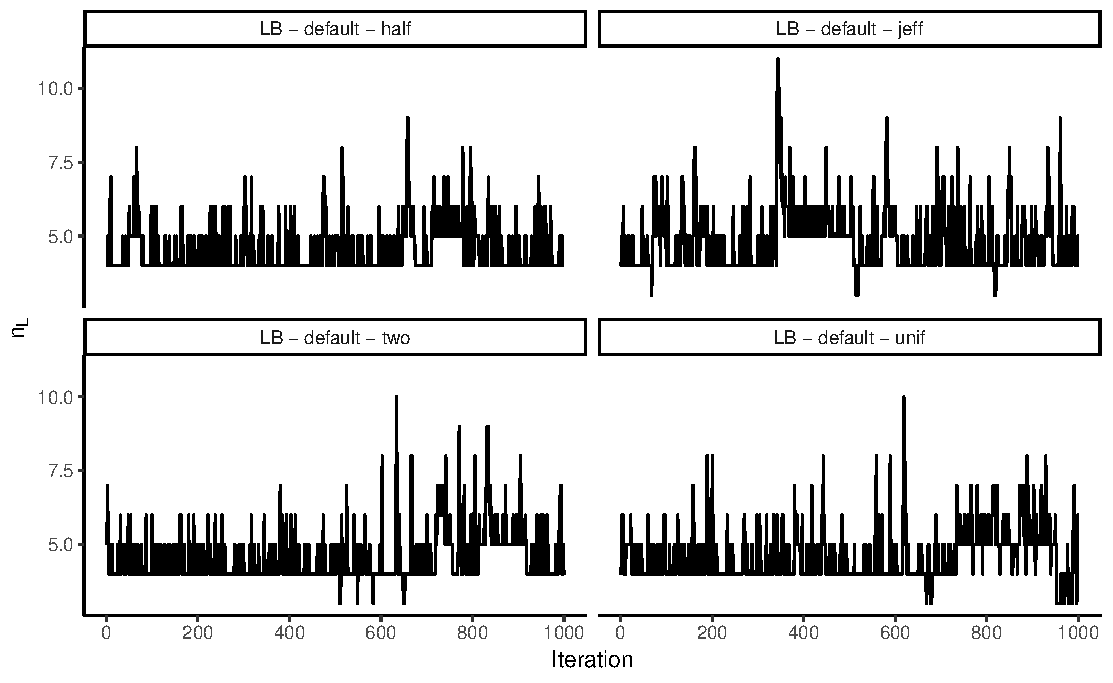
\includegraphics[width = 0.75\linewidth]{trace_case1_gauss_nterm.pdf}
	\caption{Trace plot of $n_L$ for case 1 with Gaussian copula. The top left denotes analysis with TBeta(0.5,0.5), top right denotes analysis with TBeta(0,0), bottom left denotes analysis with TBeta(2,2) and bottom right denotes analysis with TBeta(1,1).}
	\label{fig:case1:gauss:nterm}
\end{figure}

\begin{figure}
	\centering
	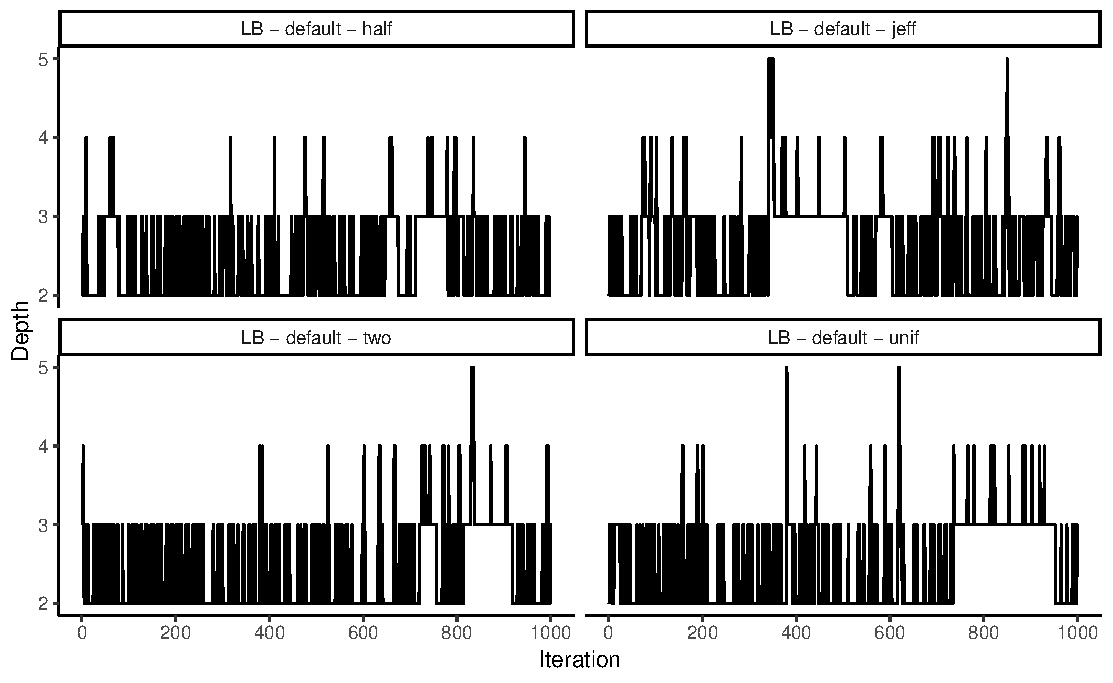
\includegraphics[width = 0.75\linewidth]{trace_case1_gauss_depth.pdf}
	\caption{Trace plot of depth for case 1 with Gaussian copula. The top left denotes analysis with TBeta(0.5,0.5), top right denotes analysis with TBeta(0,0), bottom left denotes analysis with TBeta(2,2) and bottom right denotes analysis with TBeta(1,1).}
	\label{fig:case1:gauss:depth}
\end{figure}

\begin{figure}
	\centering
	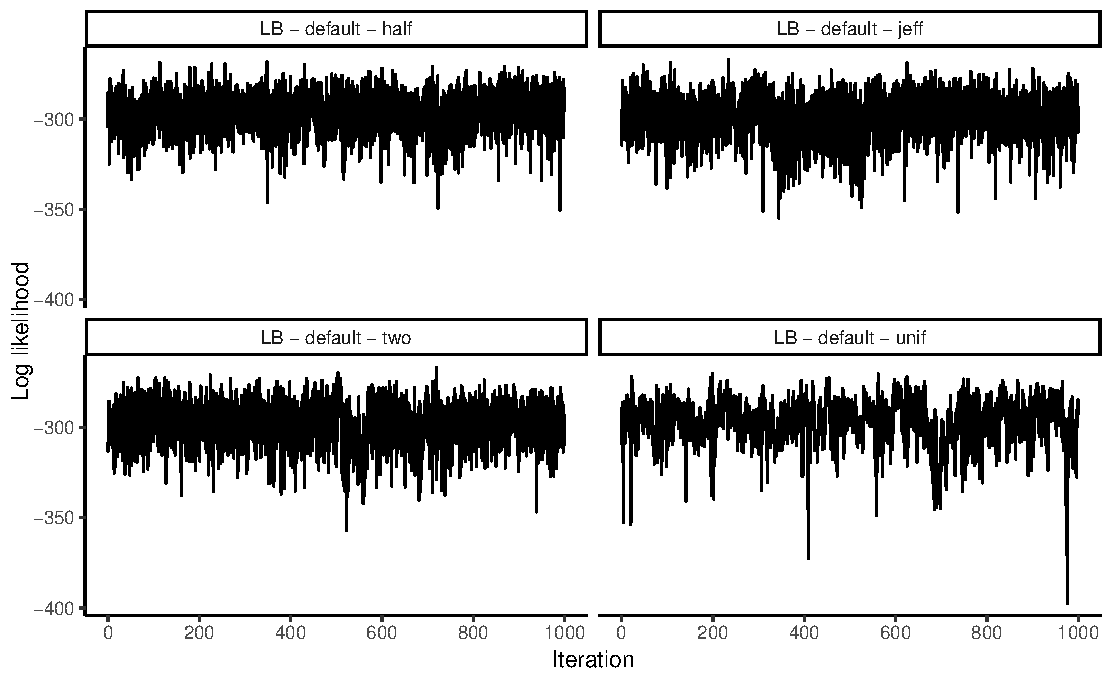
\includegraphics[width = 0.75\linewidth]{trace_case1_gauss_like.pdf}
	\caption{Trace plot of likelihood for case 1 with Gaussian copula. The top left denotes analysis with TBeta(0.5,0.5), top right denotes analysis with TBeta(0,0), bottom left denotes analysis with TBeta(2,2) and bottom right denotes analysis with TBeta(1,1).}
	\label{fig:case1:gauss:like}
\end{figure}

\begin{figure}
	\centering
	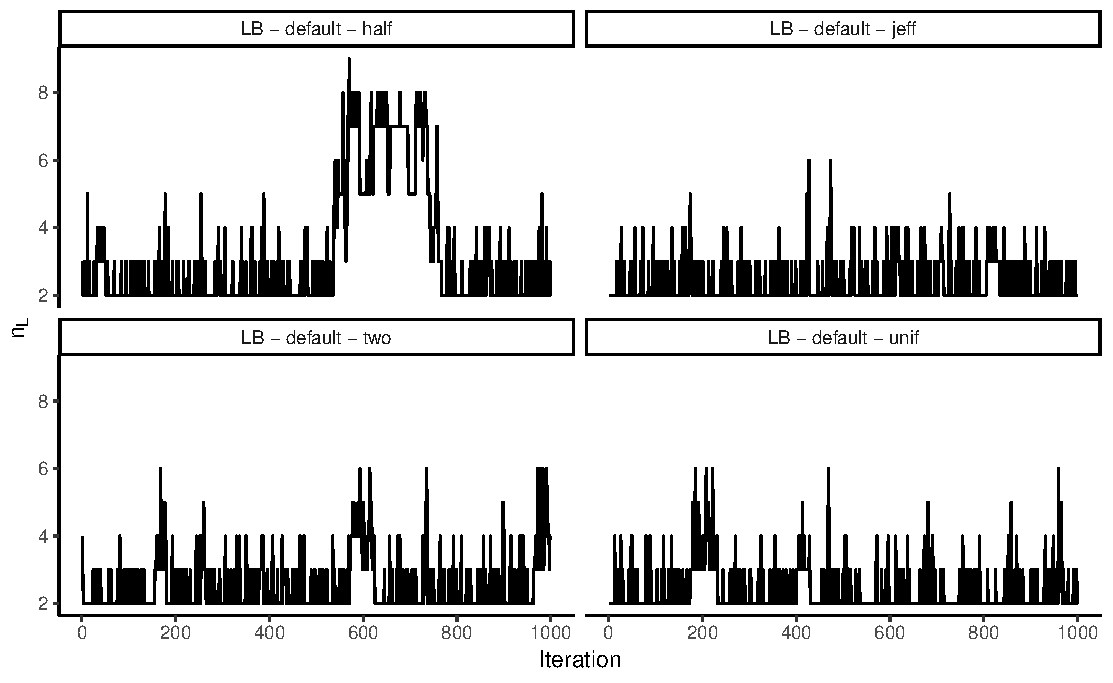
\includegraphics[width = 0.75\linewidth]{trace_case2_gauss_nterm.pdf}
	\caption{Trace plot of $n_L$ for case 2 with Gaussian copula. The top left denotes analysis with TBeta(0.5,0.5), top right denotes analysis with TBeta(0,0), bottom left denotes analysis with TBeta(2,2) and bottom right denotes analysis with TBeta(1,1).}
	\label{fig:case2:gauss:nterm}
\end{figure}

\begin{figure}
	\centering
	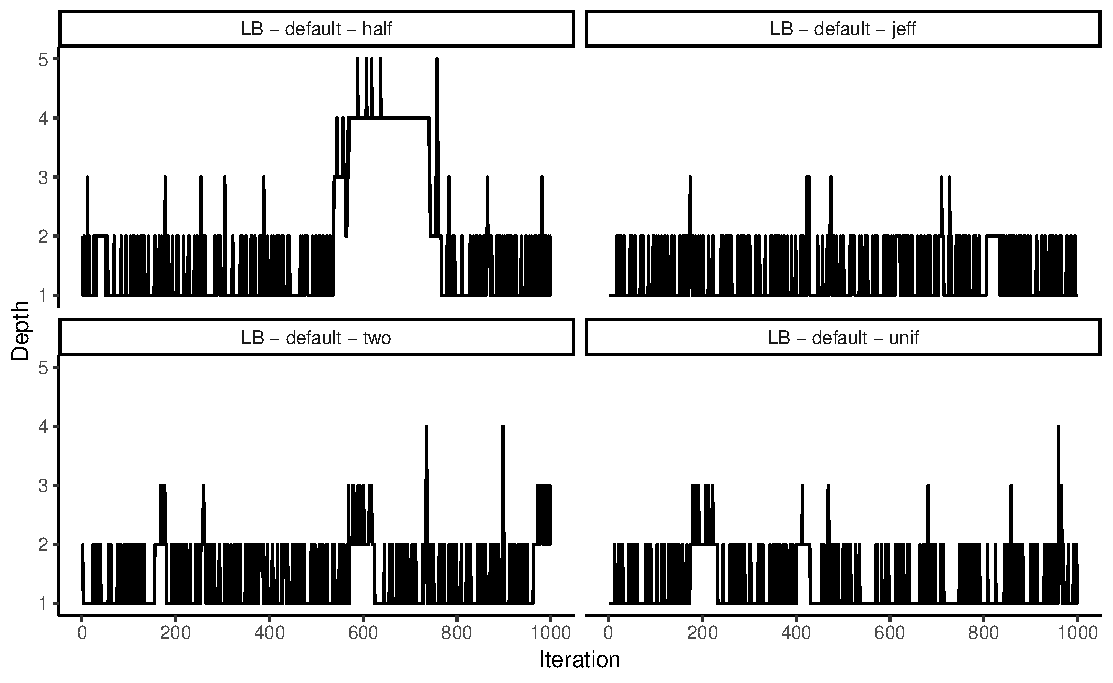
\includegraphics[width = 0.75\linewidth]{trace_case2_gauss_depth.pdf}
	\caption{Trace plot of depth for case 2 with Gaussian copula. The top left denotes analysis with TBeta(0.5,0.5), top right denotes analysis with TBeta(0,0), bottom left denotes analysis with TBeta(2,2) and bottom right denotes analysis with TBeta(1,1).}
	\label{fig:case2:gauss:depth}
\end{figure}

\begin{figure}
	\centering
	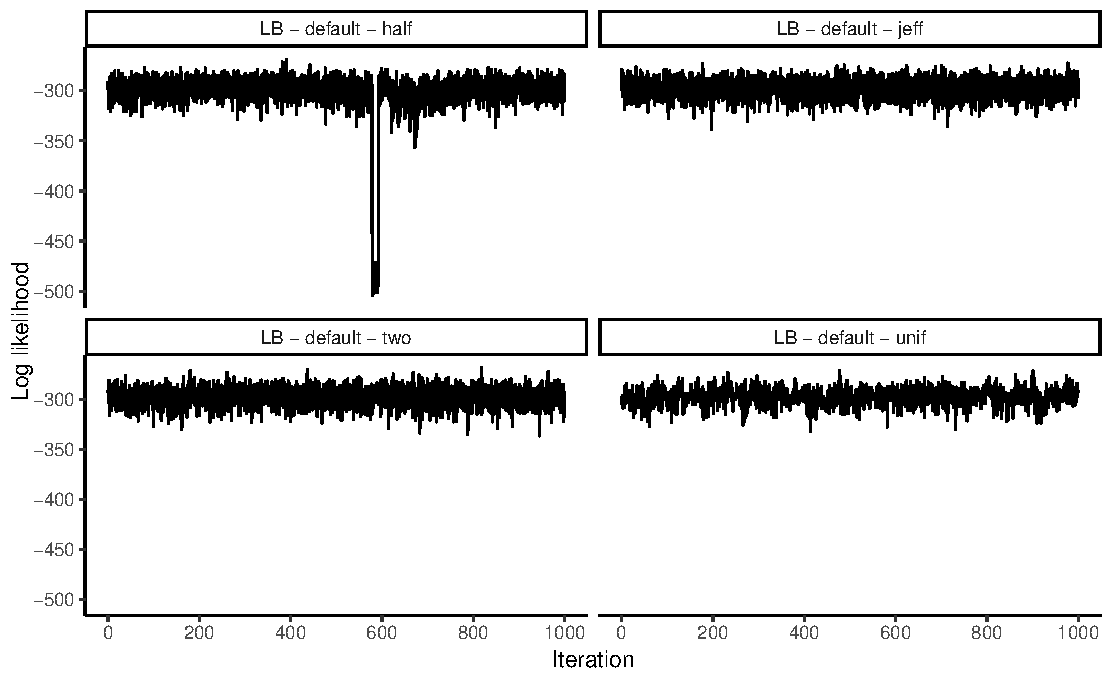
\includegraphics[width = 0.75\linewidth]{trace_case2_gauss_like.pdf}
	\caption{Trace plot of likelihood for case 2 with Gaussian copula. The top left denotes analysis with TBeta(0.5,0.5), top right denotes analysis with TBeta(0,0), bottom left denotes analysis with TBeta(2,2) and bottom right denotes analysis with TBeta(1,1).}
	\label{fig:case2:gauss:like}
\end{figure}

\begin{figure}
	\centering
	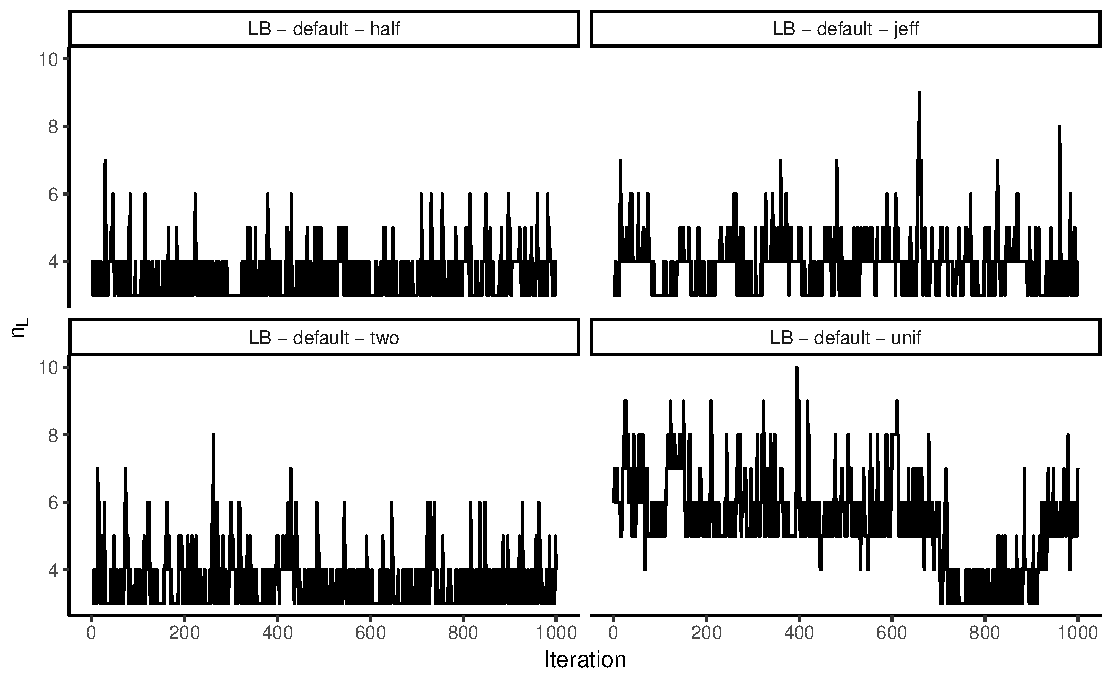
\includegraphics[width = 0.75\linewidth]{trace_case3_gauss_nterm.pdf}
	\caption{Trace plot of $n_L$ for case 3 with Gaussian copula. The top left denotes analysis with TBeta(0.5,0.5), top right denotes analysis with TBeta(0,0), bottom left denotes analysis with TBeta(2,2) and bottom right denotes analysis with TBeta(1,1).}
	\label{fig:case3:gauss:nterm}
\end{figure}

\begin{figure}
	\centering
	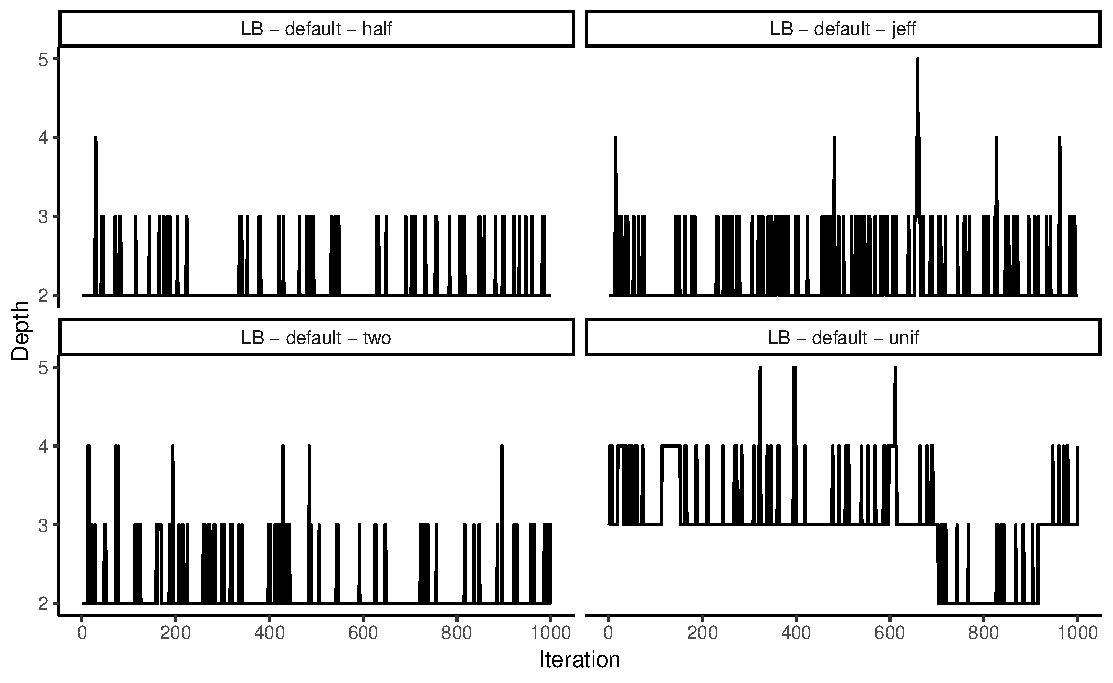
\includegraphics[width = 0.75\linewidth]{trace_case3_gauss_depth.pdf}
	\caption{Trace plot of depth for case 3 with Gaussian copula. The top left denotes analysis with TBeta(0.5,0.5), top right denotes analysis with TBeta(0,0), bottom left denotes analysis with TBeta(2,2) and bottom right denotes analysis with TBeta(1,1).}
	\label{fig:case3:gauss:depth}
\end{figure}

\begin{figure}
	\centering
	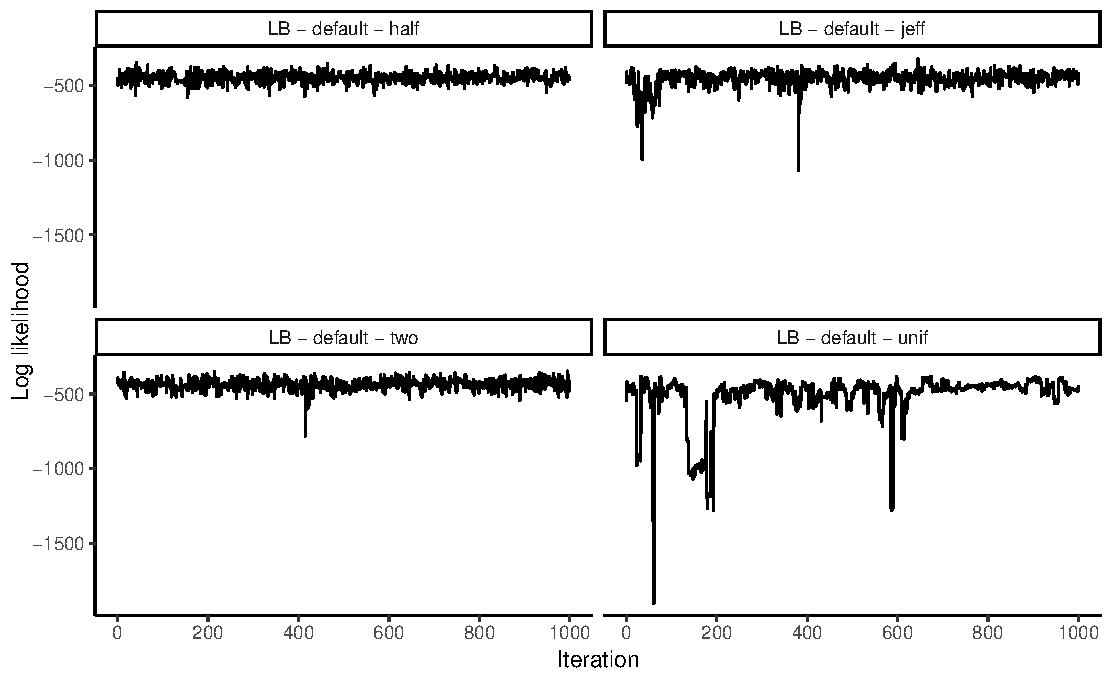
\includegraphics[width = 0.75\linewidth]{trace_case3_gauss_like.pdf}
	\caption{Trace plot of likelihood for case 3 with Gaussian copula. The top left denotes analysis with TBeta(0.5,0.5), top right denotes analysis with TBeta(0,0), bottom left denotes analysis with TBeta(2,2) and bottom right denotes analysis with TBeta(1,1).}
	\label{fig:case3:gauss:like}
\end{figure}

\begin{figure}
	\centering
	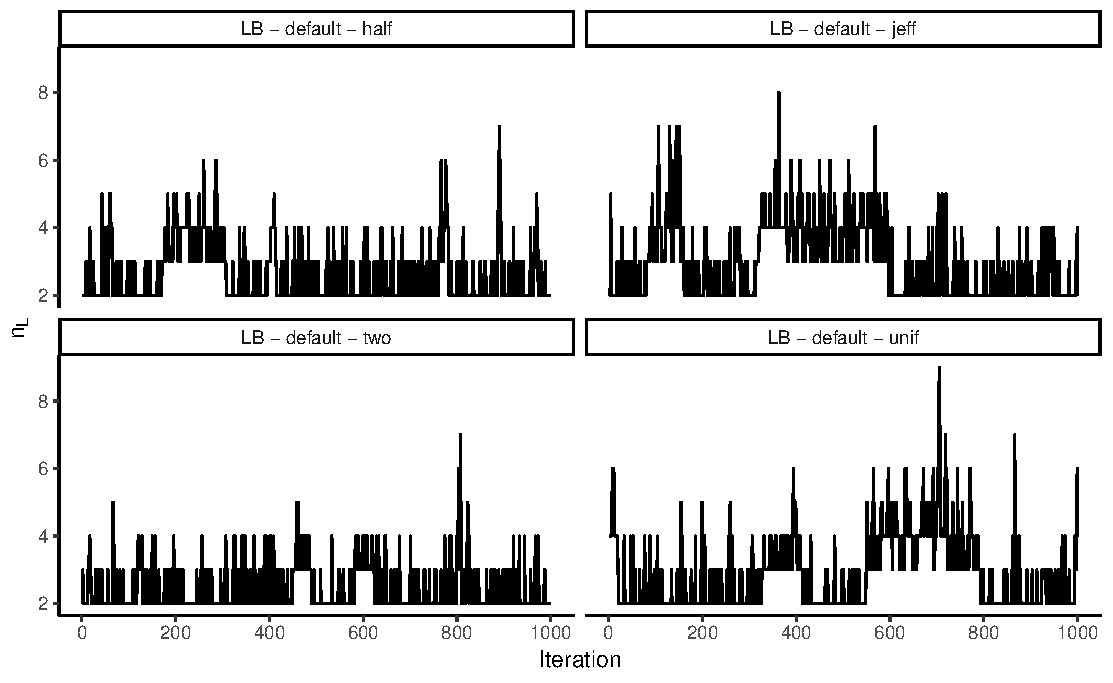
\includegraphics[width = 0.75\linewidth]{trace_case4_gauss_nterm.pdf}
	\caption{Trace plot of $n_L$ for case 4 with Gaussian copula. The top left denotes analysis with TBeta(0.5,0.5), top right denotes analysis with TBeta(0,0), bottom left denotes analysis with TBeta(2,2) and bottom right denotes analysis with TBeta(1,1).}
	\label{fig:case4:gauss:nterm}
\end{figure}

\begin{figure}
	\centering
	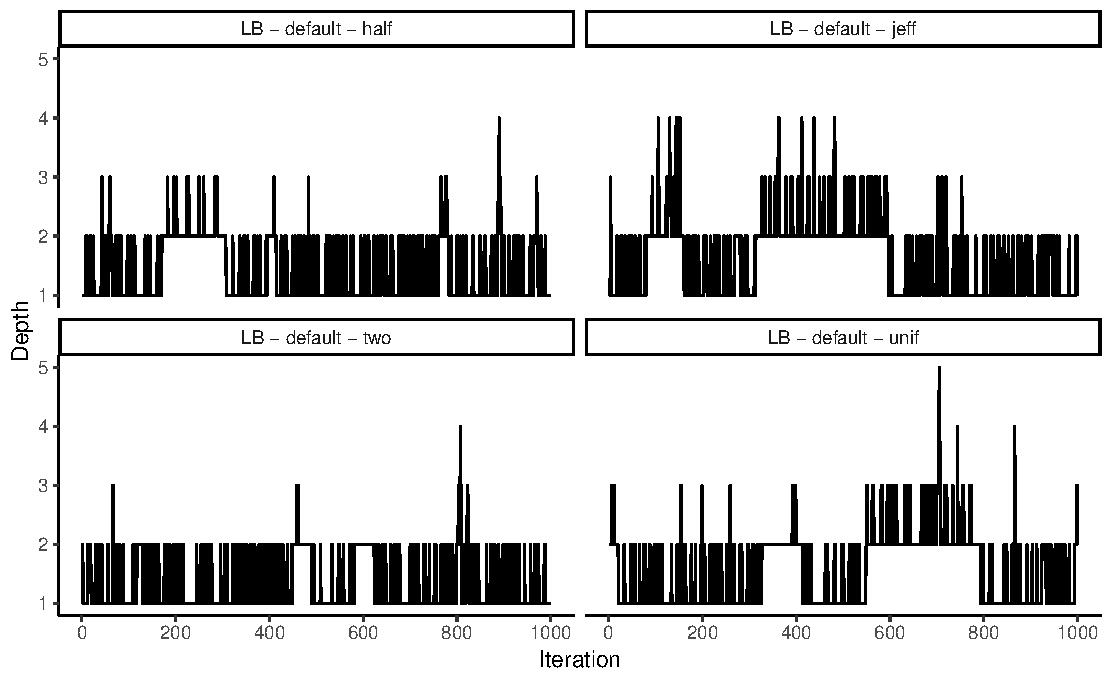
\includegraphics[width = 0.75\linewidth]{trace_case4_gauss_depth.pdf}
	\caption{Trace plot of depth for case 4 with Gaussian copula. The top left denotes analysis with TBeta(0.5,0.5), top right denotes analysis with TBeta(0,0), bottom left denotes analysis with TBeta(2,2) and bottom right denotes analysis with TBeta(1,1).}
	\label{fig:case4:gauss:depth}
\end{figure}

\begin{figure}
	\centering
	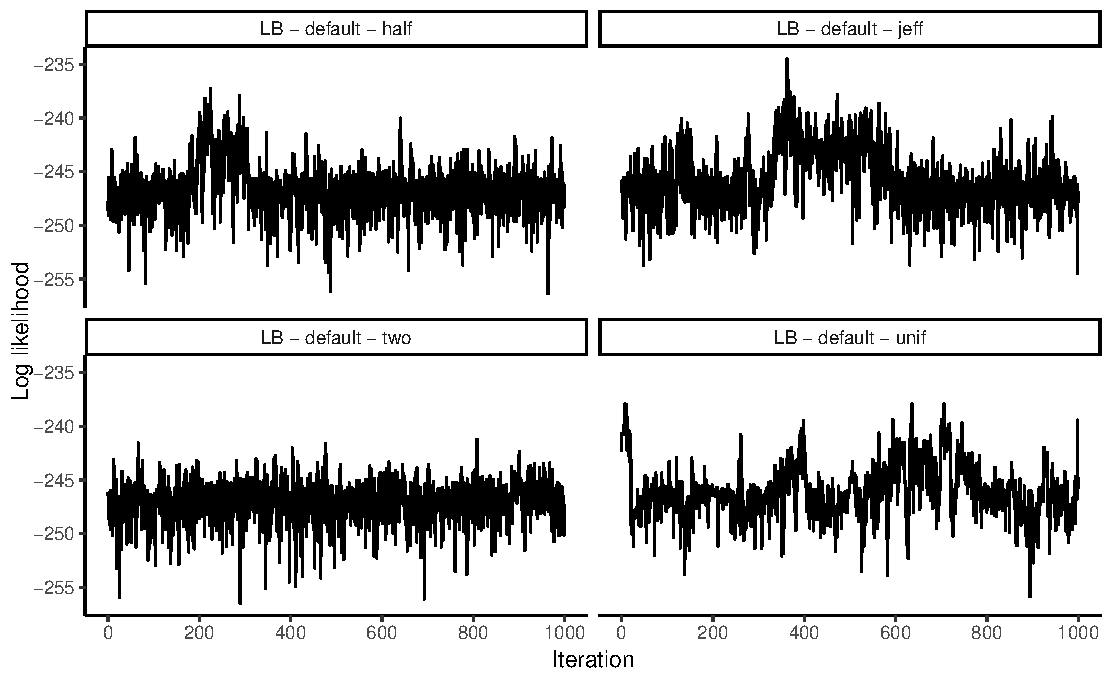
\includegraphics[width = 0.75\linewidth]{trace_case4_gauss_like.pdf}
	\caption{Trace plot of likelihood for case 4 with Gaussian copula. The top left denotes analysis with TBeta(0.5,0.5), top right denotes analysis with TBeta(0,0), bottom left denotes analysis with TBeta(2,2) and bottom right denotes analysis with TBeta(1,1).}
	\label{fig:case4:gauss:like}
\end{figure}

\subsubsection{Student-t copula} For the student-t copula we are only interested in estimating $\rho$ which lies within $(-1,1)$. Therefore, similar to Gaussian copula, we use a transformed beta distribution as a prior on $\mu_j$ with four different sets of parameters.

We present the summary of our analyses with student-t copula in \cref{tab:student-t:summary}. 


\begin{table}[ht]
	\centering
	\caption{Summary of analyses with student-t copula. The columns represents the specific case, the type of prior on $\mu_j\mid T$, the posterior expected number of terminal nodes, the posterior expected depth, the acceptance rate of MH algorithm, RMSE of estimated $\rho$ against true $\rho$, length of credible interval and coverage frequency within the credible interval. The posterior quantities are obtained by running 15000 samples in a single chain, after that we remove 5000 samples and then by thinned by 10.}
	\label{tab:student-t:summary}
	\scriptsize{
	\begin{tabular}{ll|cccccc}
		\toprule
		& Prior on $\mu_j$ & $\mathbb{E}(n_L\mid U,X)$ & $\mathbb{E}(D\mid U,X)$ & Acc. Rate & RMSE & CI length & CI coverage \\ 
		\midrule
		Case 1 & TBeta(0.5,0.5) & 3.370 & 1.884 & 0.251 & 0.0079 & 0.2277 & 0.860 \\ 
		(Tree) & TBeta(0,0) & 4.089 & 2.228 & 0.268 & 0.0072 & 0.2445 & 0.850 \\ 
		& TBeta(2,2) & 3.620 & 2.041 & 0.260 & 0.0080 & 0.2420 & \textbf{0.862} \\ 
		& TBeta(1,1) & 3.604 & 1.996 & 0.232 & 0.0080 & 0.2308 & 0.854 \\ 
		\midrule
		Case 2 & TBeta(0.5,0.5) & 2.394 & 1.311 & 0.246 & 0.0019 & 0.1980 & \textbf{1.000} \\ 
		(\cref{eq:synth:tau_x:case2}) & TBeta(0,0) & 2.326 & 1.255 & 0.203 & 0.0018 & 0.2000 & \textbf{1.000} \\ 
		& TBeta(2,2) & 2.470 & 1.351 & 0.236 & 0.0019 & 0.2115 & \textbf{1.000} \\ 
		& TBeta(1,1) & 2.354 & 1.289 & 0.213 & 0.0018 & 0.1950 & \textbf{1.000} \\ 
		\midrule
		Case 3 & TBeta(0.5,0.5) & 3.499 & 2.102 & 0.261 & 0.0008 & 0.0997 & 0.916 \\ 
		(\cref{eq:synth:tau_x:case3}) & TBeta(0,0) & 3.727 & 2.170 & 0.261 & 0.0007 & 0.0992 & 0.928 \\ 
		& TBeta(2,2) & 3.545 & 2.127 & 0.238 & 0.0007 & 0.1127 & 0.896 \\ 
		& TBeta(1,1) & 3.847 & 2.234 & 0.243 & 0.0008 & 0.0971 & \textbf{0.950} \\ 
		\midrule
		Case 4 & TBeta(0.5,0.5) & 2.560 & 1.431 & 0.241 & 0.0003 & 0.1552 & \textbf{1.000} \\ 
		(\cref{eq:synth:tau_x:case4}) & TBeta(0,0) & 2.387 & 1.311 & 0.275 & 0.0003 & 0.1406 & \textbf{1.000} \\ 
		& TBeta(2,2) & 2.689 & 1.488 & 0.266 & 0.0003 & 0.1648 & \textbf{1.000} \\ 
		& TBeta(1,1) & 2.824 & 1.568 & 0.259 & 0.0003 & 0.1482 & \textbf{1.000} \\ 
		\end{tabular}}
\end{table}

\paragraph{Trace-plots}

\begin{figure}
	\centering
	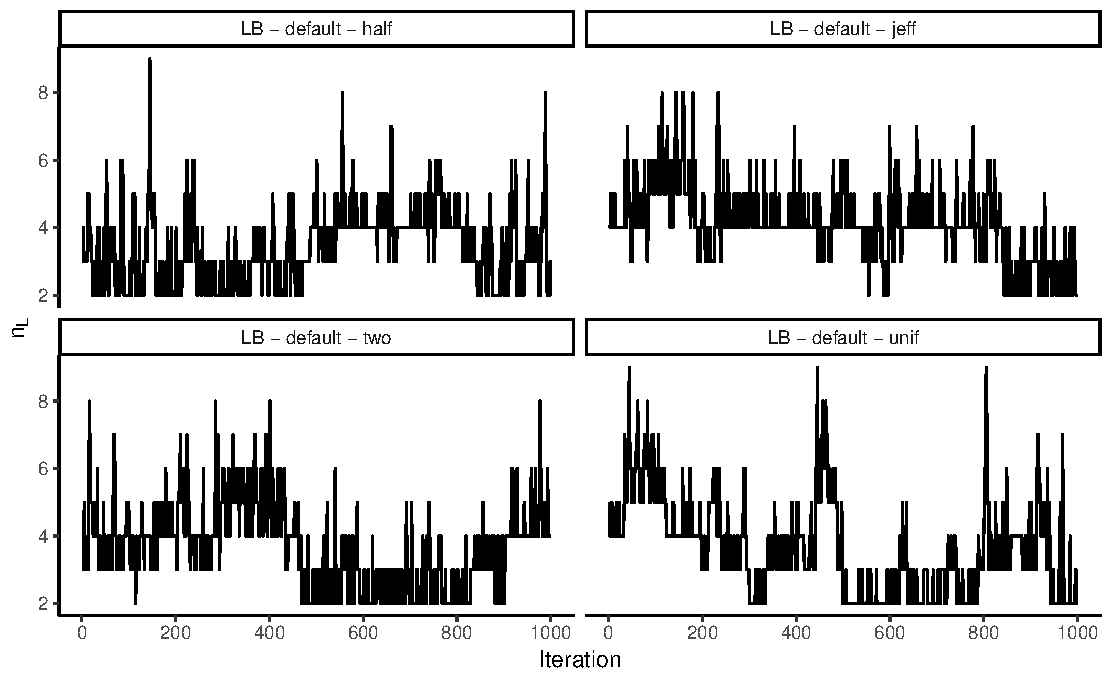
\includegraphics[width = 0.75\linewidth]{trace_case1_t_nterm.pdf}
	\caption{Trace plot of $n_L$ for case 1 with t copula. The top left denotes analysis with TBeta(0.5,0.5), top right denotes analysis with TBeta(0,0), bottom left denotes analysis with TBeta(2,2) and bottom right denotes analysis with TBeta(1,1).}
	\label{fig:case1:t:nterm}
\end{figure}

\begin{figure}
	\centering
	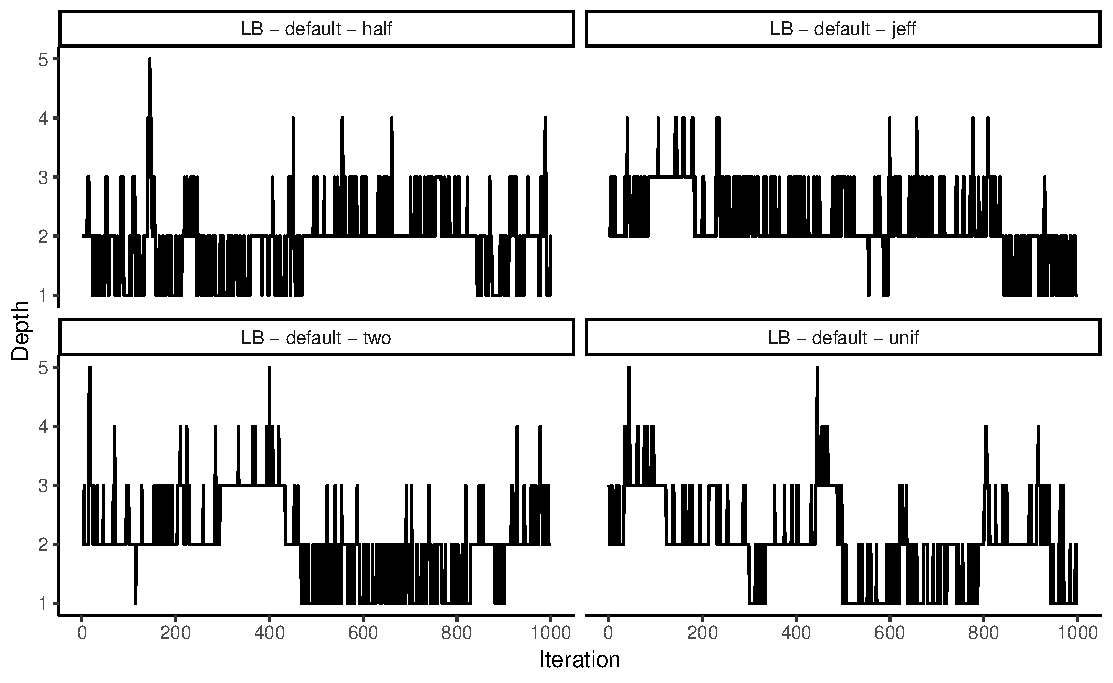
\includegraphics[width = 0.75\linewidth]{trace_case1_t_depth.pdf}
	\caption{Trace plot of depth for case 1 with t copula. The top left denotes analysis with TBeta(0.5,0.5), top right denotes analysis with TBeta(0,0), bottom left denotes analysis with TBeta(2,2) and bottom right denotes analysis with TBeta(1,1).}
	\label{fig:case1:t:depth}
\end{figure}

\begin{figure}
	\centering
	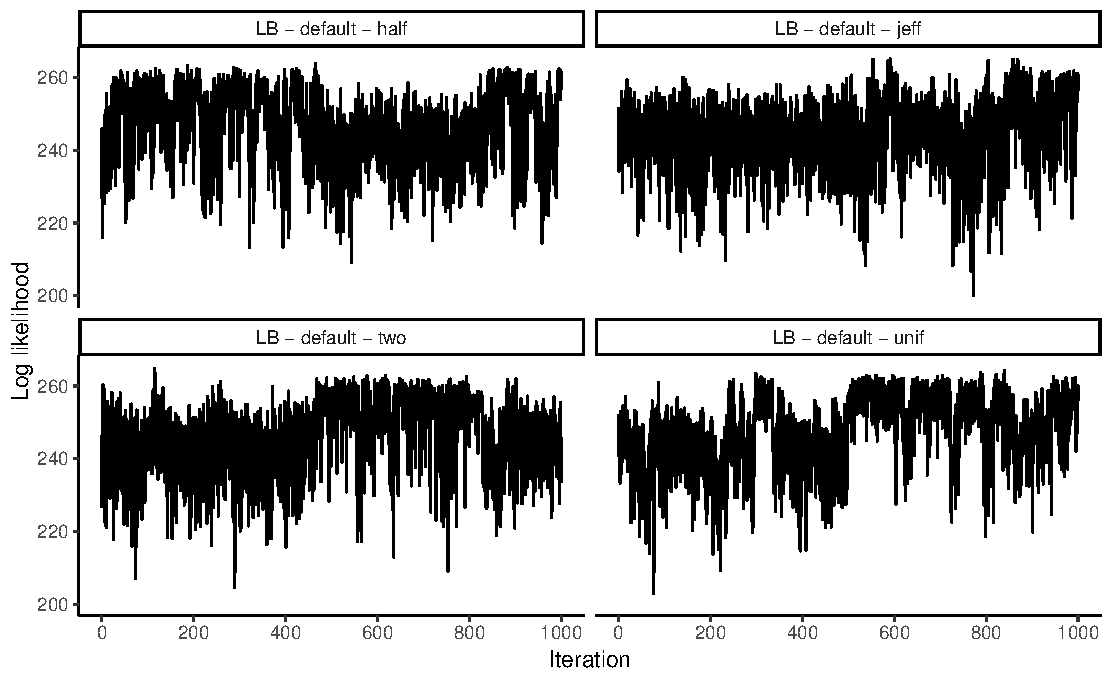
\includegraphics[width = 0.75\linewidth]{trace_case1_t_like.pdf}
	\caption{Trace plot of likelihood for case 1 with t copula. The top left denotes analysis with TBeta(0.5,0.5), top right denotes analysis with TBeta(0,0), bottom left denotes analysis with TBeta(2,2) and bottom right denotes analysis with TBeta(1,1).}
	\label{fig:case1:t:like}
\end{figure}

\begin{figure}
	\centering
	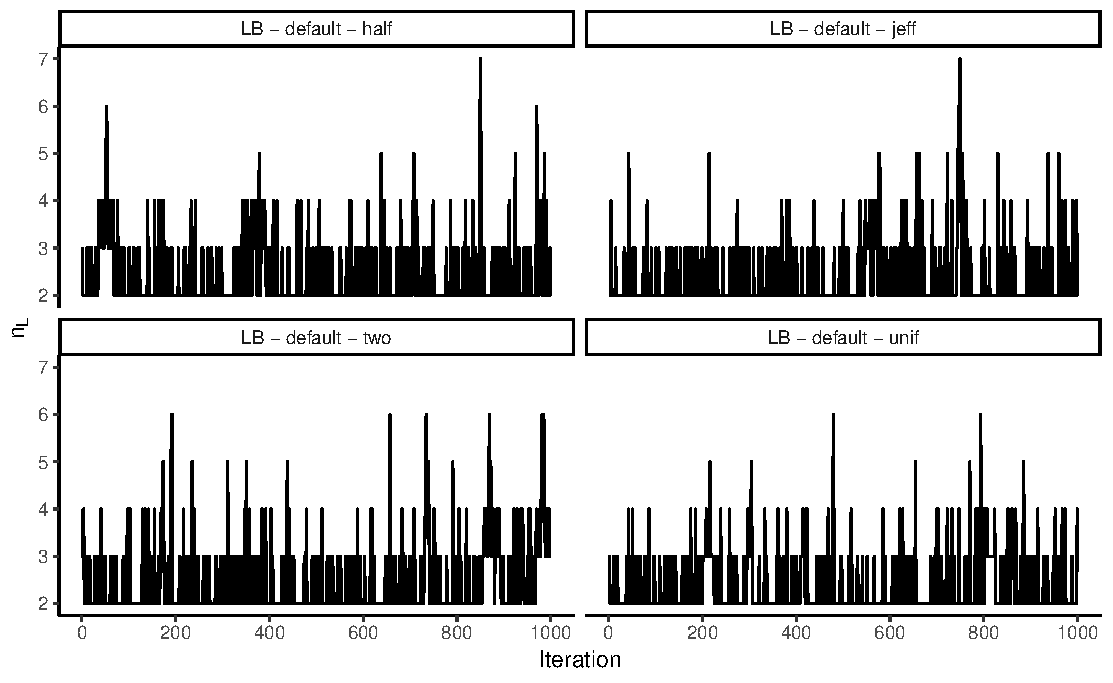
\includegraphics[width = 0.75\linewidth]{trace_case2_t_nterm.pdf}
	\caption{Trace plot of $n_L$ for case 2 with t copula. The top left denotes analysis with TBeta(0.5,0.5), top right denotes analysis with TBeta(0,0), bottom left denotes analysis with TBeta(2,2) and bottom right denotes analysis with TBeta(1,1).}
	\label{fig:case2:t:nterm}
\end{figure}

\begin{figure}
	\centering
	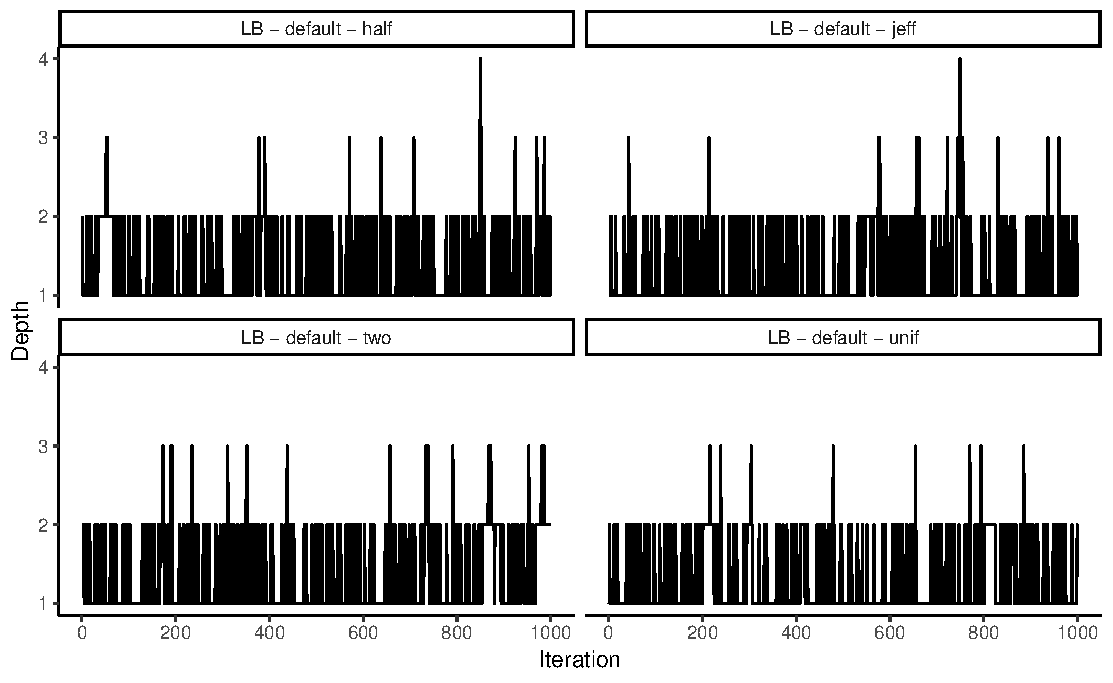
\includegraphics[width = 0.75\linewidth]{trace_case2_t_depth.pdf}
	\caption{Trace plot of depth for case 2 with t copula. The top left denotes analysis with TBeta(0.5,0.5), top right denotes analysis with TBeta(0,0), bottom left denotes analysis with TBeta(2,2) and bottom right denotes analysis with TBeta(1,1).}
	\label{fig:case2:t:depth}
\end{figure}

\begin{figure}
	\centering
	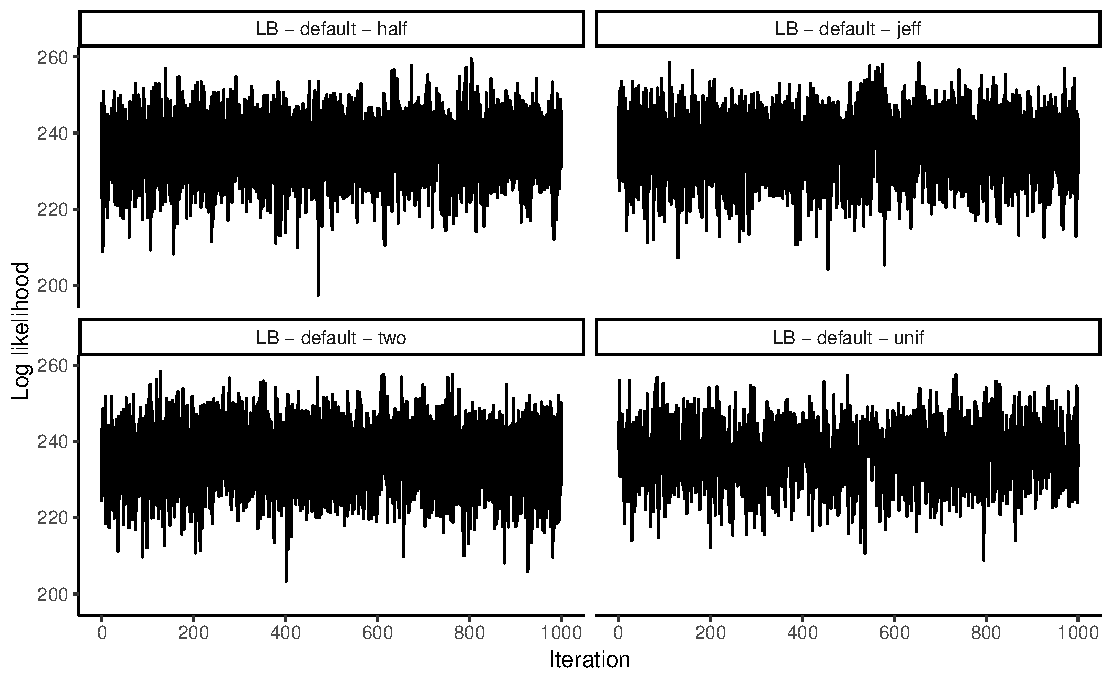
\includegraphics[width = 0.75\linewidth]{trace_case2_t_like.pdf}
	\caption{Trace plot of likelihood for case 2 with t copula. The top left denotes analysis with TBeta(0.5,0.5), top right denotes analysis with TBeta(0,0), bottom left denotes analysis with TBeta(2,2) and bottom right denotes analysis with TBeta(1,1).}
	\label{fig:case2:t:like}
\end{figure}

\begin{figure}
	\centering
	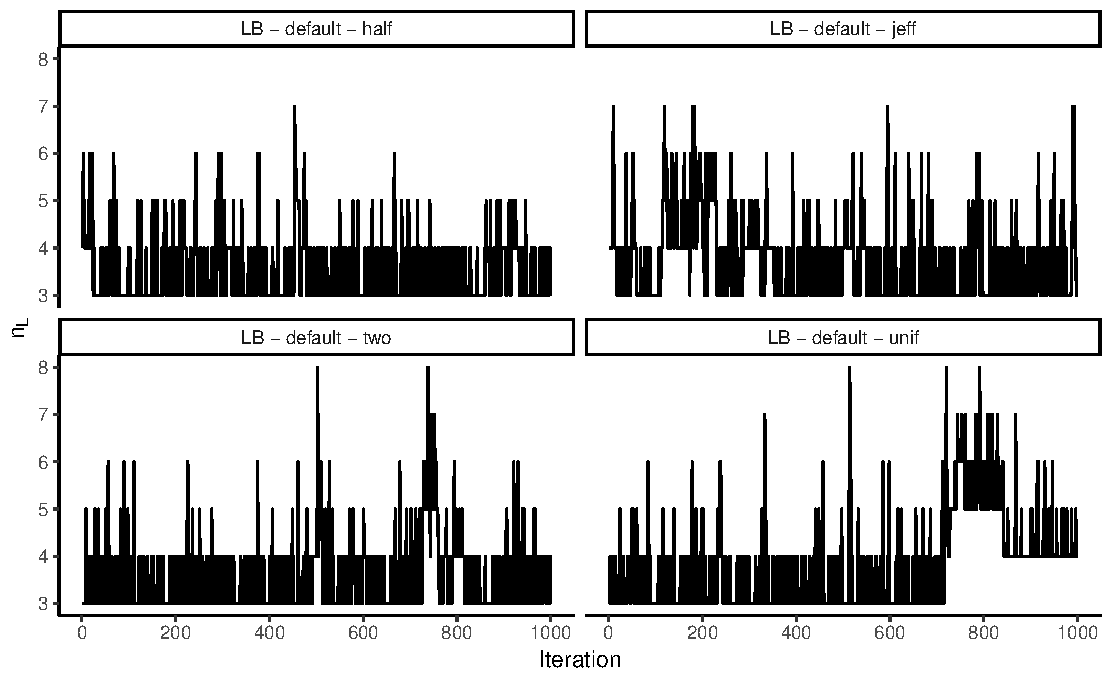
\includegraphics[width = 0.75\linewidth]{trace_case3_t_nterm.pdf}
	\caption{Trace plot of $n_L$ for case 3 with t copula. The top left denotes analysis with TBeta(0.5,0.5), top right denotes analysis with TBeta(0,0), bottom left denotes analysis with TBeta(2,2) and bottom right denotes analysis with TBeta(1,1).}
	\label{fig:case3:t:nterm}
\end{figure}

\begin{figure}
	\centering
	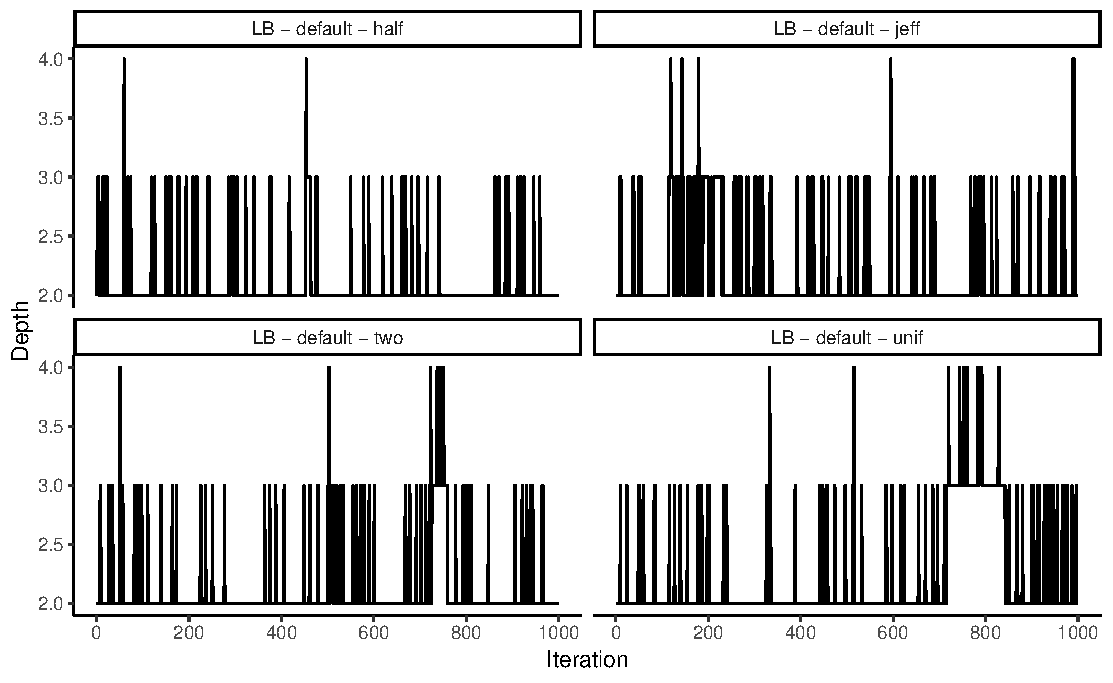
\includegraphics[width = 0.75\linewidth]{trace_case3_t_depth.pdf}
	\caption{Trace plot of depth for case 3 with t copula. The top left denotes analysis with TBeta(0.5,0.5), top right denotes analysis with TBeta(0,0), bottom left denotes analysis with TBeta(2,2) and bottom right denotes analysis with TBeta(1,1).}
	\label{fig:case3:t:depth}
\end{figure}

\begin{figure}
	\centering
	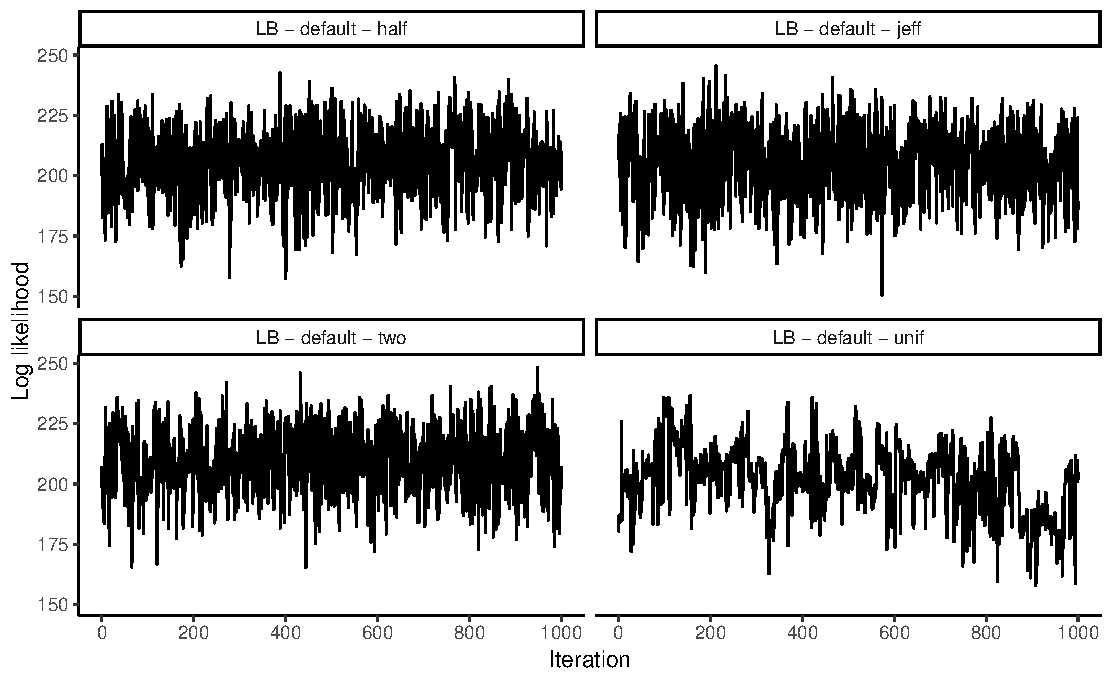
\includegraphics[width = 0.75\linewidth]{trace_case3_t_like.pdf}
	\caption{Trace plot of likelihood for case 3 with t copula. The top left denotes analysis with TBeta(0.5,0.5), top right denotes analysis with TBeta(0,0), bottom left denotes analysis with TBeta(2,2) and bottom right denotes analysis with TBeta(1,1).}
	\label{fig:case3:t:like}
\end{figure}

\begin{figure}
	\centering
	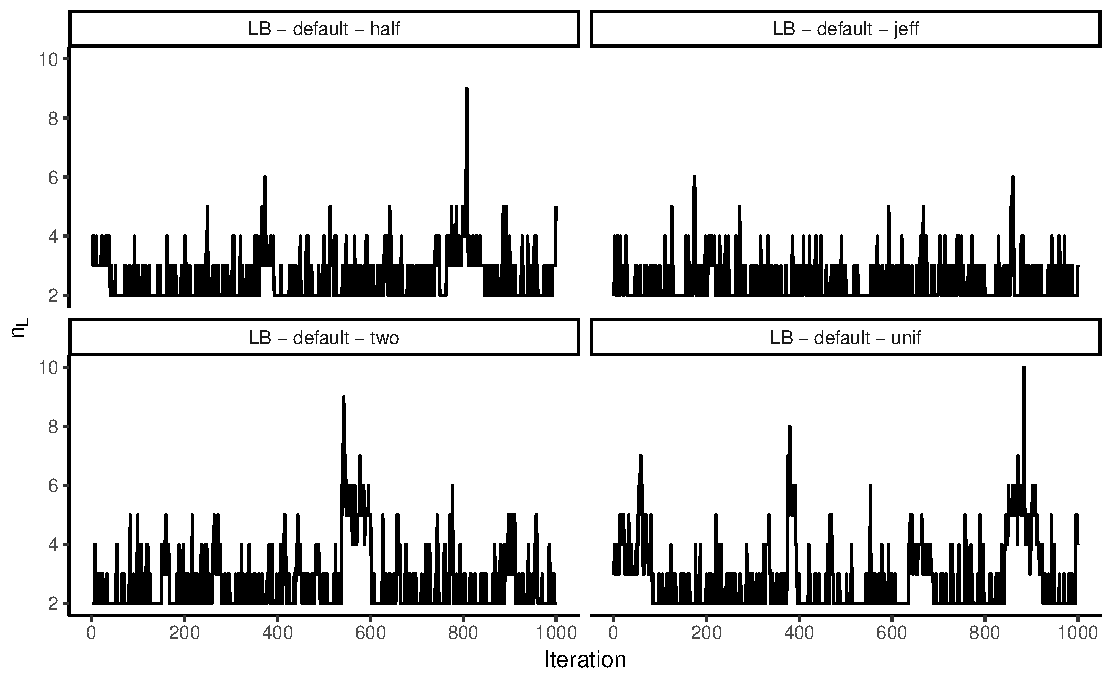
\includegraphics[width = 0.75\linewidth]{trace_case4_t_nterm.pdf}
	\caption{Trace plot of $n_L$ for case 4 with t copula. The top left denotes analysis with TBeta(0.5,0.5), top right denotes analysis with TBeta(0,0), bottom left denotes analysis with TBeta(2,2) and bottom right denotes analysis with TBeta(1,1).}
	\label{fig:case4:t:nterm}
\end{figure}

\begin{figure}
	\centering
	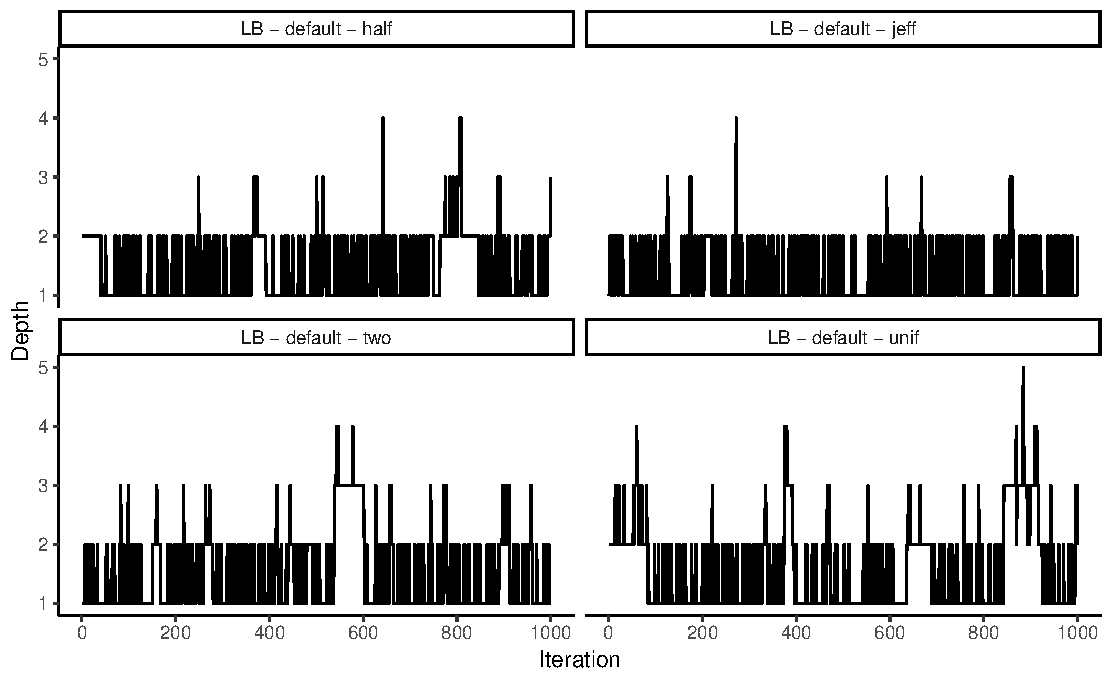
\includegraphics[width = 0.75\linewidth]{trace_case4_t_depth.pdf}
	\caption{Trace plot of depth for case 4 with t copula. The top left denotes analysis with TBeta(0.5,0.5), top right denotes analysis with TBeta(0,0), bottom left denotes analysis with TBeta(2,2) and bottom right denotes analysis with TBeta(1,1).}
	\label{fig:case4:t:depth}
\end{figure}

\begin{figure}
	\centering
	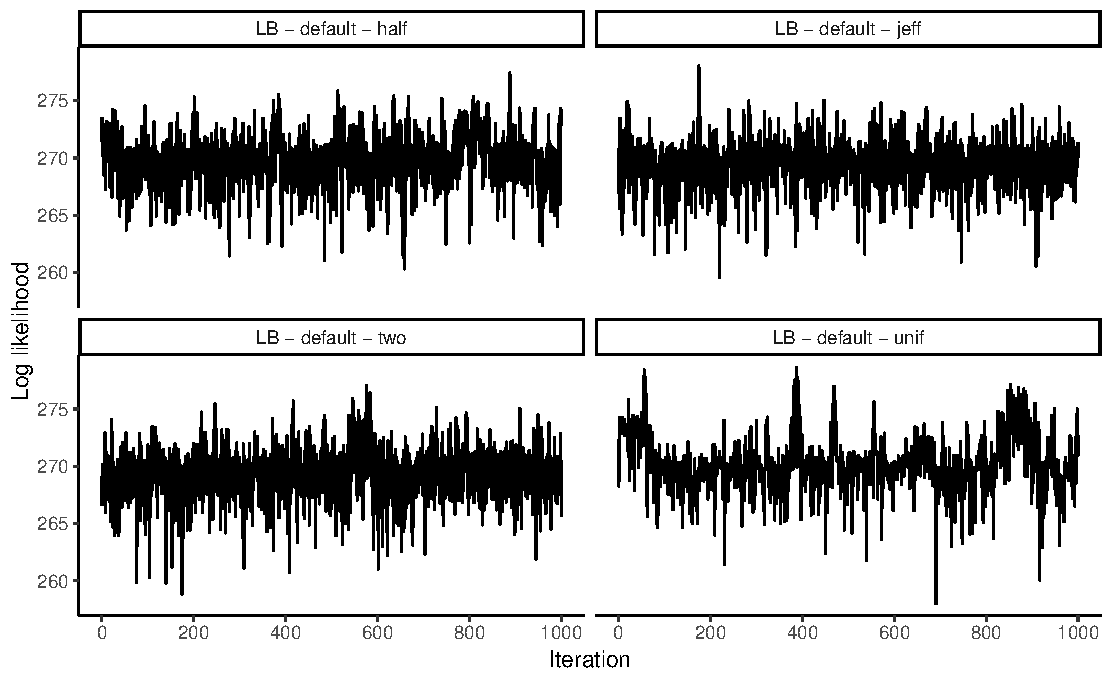
\includegraphics[width = 0.75\linewidth]{trace_case4_t_like.pdf}
	\caption{Trace plot of likelihood for case 4 with t copula. The top left denotes analysis with TBeta(0.5,0.5), top right denotes analysis with TBeta(0,0), bottom left denotes analysis with TBeta(2,2) and bottom right denotes analysis with TBeta(1,1).}
	\label{fig:case4:t:like}
\end{figure}

\subsubsection{Clayton copula} The copula parameter of the Gumbel copula lies in the open interval $(0,\infty)$. So we consider log-normal and gamma distribution for $\mu_j$

We present the summary of our analyses with Clayton copula in \cref{tab:clayton:summary}. 


\begin{table}[ht]
	\centering
	\caption{Summary of analyses with Clayton copula. The columns represents the specific case, the type of prior on $\mu_j\mid T$, the posterior expected number of terminal nodes, the posterior expected depth, the acceptance rate of MH algorithm, RMSE of estimated $\theta$ against true $\theta$, length of credible interval and coverage frequency within the credible interval. The posterior quantities are obtained by running 15000 samples in a single chain, after that we remove 5000 samples and then by thinned by 10.}
	\label{tab:clayton:summary}
	\scriptsize{
		\begin{tabular}{ll|cccccc}
			\toprule
			& Prior on $\mu_j$ & $\mathbb{E}(n_L\mid U,X)$ & $\mathbb{E}(D\mid U,X)$ & Acc. Rate & RMSE & CI length & CI coverage \\ 
			\midrule
			Case 1 & Gamma(1,1) & 2.867 & 1.662 & 0.232 & 0.5097 & 1.3417 & 0.764 \\ 
			(Tree) & Gamma(2,2) & 4.246 & 2.416 & 0.300 & 0.3705 & 1.5866 & \textbf{0.924} \\ 
			& LogNorm(0,1) & 3.629 & 2.095 & 0.285 & 0.4099 & 1.5664 & 0.824 \\ 
			& LogNorm(0,5) & 3.876 & 2.178 & 0.246 & 0.3598 & 1.7381 & 0.842 \\ 
			\midrule
			Case 2 & Gamma(1,1) & 2.291 & 1.228 & 0.202 & 0.1254 & 0.9802 & 0.880 \\ 
			(\cref{eq:synth:tau_x:case2}) & Gamma(2,2) & 2.703 & 1.513 & 0.245 & 0.0902 & 1.2297 & \textbf{1.000} \\ 
			& LogNorm(0,1) & 2.799 & 1.581 & 0.249 & 0.0757 & 1.2844 & \textbf{1.000} \\ 
			& LogNorm(0,5) & 2.625 & 1.467 & 0.213 & 0.0834 & 1.2934 & \textbf{1.000} \\ 
			\midrule
			Case 3 & Gamma(1,1) & 3.388 & 2.060 & 0.229 & 0.6166 & 2.2269 & 0.754 \\ 
			(\cref{eq:synth:tau_x:case3}) & Gamma(2,2) & 3.588 & 2.125 & 0.259 & 0.5407 & 2.5436 & 0.822 \\ 
			& LogNorm(0,1) & 3.679 & 2.147 & 0.232 & 0.5492 & 2.4543 & \textbf{0.902} \\ 
			& LogNorm(0,5) & 3.516 & 2.111 & 0.265 & 0.5881 & 2.4645 & 0.884 \\ 
			\midrule
			Case 4 & Gamma(1,1) & 2.205 & 1.183 & 0.207 & 0.0492 & 1.0143 & \textbf{0.978} \\ 
			(\cref{eq:synth:tau_x:case4}) & Gamma(2,2) & 2.318 & 1.260 & 0.214 & 0.0527 & 1.0409 & 0.974 \\ 
			& LogNorm(0,1) & 2.377 & 1.301 & 0.241 & 0.0531 & 1.0920 & 0.972 \\ 
			& LogNorm(0,5) & 2.407 & 1.320 & 0.204 & 0.0561 & 1.1192 & 0.974 \\ 
	\end{tabular}}
\end{table}


\subsubsection{Gumbel copula} The copula parameter of the Gumbel copula lies in the open interval $[1,\infty)$. So we consider log-normal and gamma distribution for $\mu_j$.

We present the summary of our analyses with Gumbel copula in \cref{tab:gumbel:summary}. 


\begin{table}[ht]
	\centering
	\caption{Summary of analyses with Gumbel copula. The columns represents the specific case, the type of prior on $\mu_j\mid T$, the posterior expected number of terminal nodes, the posterior expected depth, the acceptance rate of MH algorithm, RMSE of estimated $\theta$ against true $\theta$, length of credible interval and coverage frequency within the credible interval. The posterior quantities are obtained by running 15000 samples in a single chain, after that we remove 5000 samples and then by thinned by 10.}
	\label{tab:gumbel:summary}
	\scriptsize{
	\begin{tabular}{ll|cccccc}
		\toprule
		& Prior on $\mu_j$ & $\mathbb{E}(n_L\mid U,X)$ & $\mathbb{E}(D\mid U,X)$ & Acc. Rate & RMSE & CI length & CI coverage \\ 
		\hline
		Case 1 & Gamma(1,1) & 4.513 & 2.397 & 0.246 & 0.1292 & 0.9088 & 0.908 \\ 
		(Tree) & Gamma(2,2) & 4.714 & 2.532 & 0.256 & 0.1407 & 0.8179 & 0.858 \\ 
		& LogNorm(0,1) & 4.626 & 2.525 & 0.260 & 0.1321 & 0.9956 & \textbf{0.916} \\ 
		& LogNorm(0,5) & 4.389 & 2.335 & 0.227 & 0.1353 & 0.8653 & 0.856 \\ 
		\midrule
		Case 2 & Gamma(1,1) & 2.373 & 1.289 & 0.202 & 0.0277 & 0.6032 & 0.998 \\ 
		(\cref{eq:synth:tau_x:case2}) & Gamma(2,2) & 2.605 & 1.455 & 0.209 & 0.0262 & 0.6956 & \textbf{1.000} \\ 
		& LogNorm(0,1) & 2.349 & 1.268 & 0.214 & 0.0273 & 0.6049 & 0.994 \\ 
		& LogNorm(0,5) & 2.408 & 1.314 & 0.212 & 0.0277 & 0.6025 & 0.974 \\ 
		\midrule
		Case 3 & Gamma(1,1) & 3.421 & 2.086 & 0.241 & 0.1523 & 1.1744 & 0.764 \\ 
		(\cref{eq:synth:tau_x:case3}) & Gamma(2,2) & 3.429 & 2.077 & 0.252 & 0.1509 & 1.2093 & 0.788 \\ 
		& LogNorm(0,1) & 3.631 & 2.173 & 0.267 & 0.1566 & 1.1954 & 0.792 \\ 
		& LogNorm(0,5) & 3.590 & 2.119 & 0.262 & 0.1575 & 1.2772 & \textbf{0.854} \\ 
		\midrule
		Case 4 & Gamma(1,1) & 2.706 & 1.517 & 0.247 & 0.0152 & 0.7585 & 0.974 \\ 
		(\cref{eq:synth:tau_x:case4}) & Gamma(2,2) & 2.602 & 1.466 & 0.252 & 0.0140 & 0.7451 & 0.974 \\ 
		& LogNorm(0,1) & 2.527 & 1.405 & 0.224 & 0.0161 & 0.7377 & 0.988 \\ 
		& LogNorm(0,5) & 2.445 & 1.353 & 0.217 & 0.0148 & 0.7090 & \textbf{0.990} \\ 
		\end{tabular}}
\end{table}


\bibliographystyle{plainnat}
\bibliography{example}

\end{document}
